\chapter{Attacks}

In this chapter we're describing the attacks that we want to simulate using
INTO-CPS\@. The attacks that we have developed are in the two variants seen
during the course:

\begin{itemize}
	\item Control: Attacks that are implemented changing the code of the
		Controller FMU\@.
	\item FMU\@: Attacks implemented using additional FMUs placed between
		two legitimate FMUs.
\end{itemize}

We have developed 6 attacks, 3 for each variant. The attacks on the control FMU
are the following:

\begin{itemize}
	\item Actuator Control Attack;
	\item Complementary Attack;
	\item Switch Sensors Attack.
\end{itemize}

The attacks with additional FMUs are the following:

\begin{itemize}
	\item Actuator Scale Attack;
	\item Max Speed Attack;
	\item Sensor Output Attack.
\end{itemize}

\section{Control Algorithm Attacks}

These attacks are, as said before, carried out modifying the control algorithm
in the controller FMU\@.

\begin{figure}[htp]
	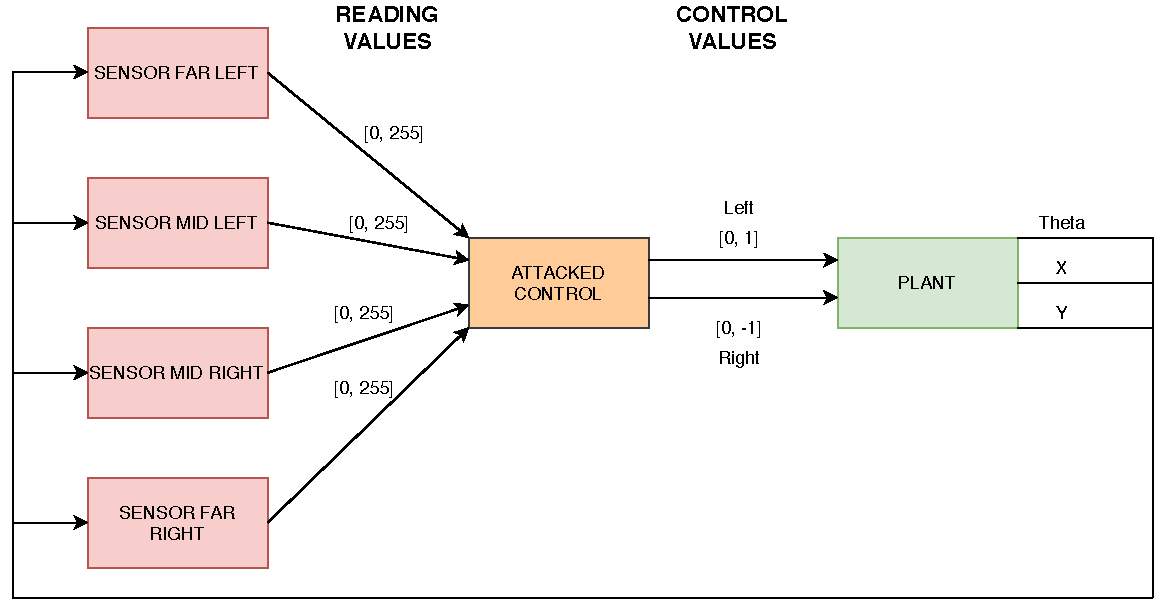
\includegraphics[width=\textwidth]{ctrl-attacks-diagram}
	\caption{Control attacks diagram}\label{fig:ctrlatksdiagram}
\end{figure}

In these section we will describe the attacks and discuss the outcomes.

\subsection{Actuator Control Attack}

This attack is implemented modifying the control algorithm inside the
\code{controller} FMU\@.

The attacker can choose some parameters:
\begin{itemize}
\item Real attack\_time: The time at which the attack starts.
\item Real attack\_duration: The duration, of the attack.
\end{itemize}

The objective of the attack is to set the input values for the actuators,
periodically, making the LFR go backward for an amount of time specified by
\code{attack\_duration} starting from \code{attack\_time}.

The control algorithm invoke the \code{actuator\_attack(State* st)} function at
the end of the \code{tick(State* st)} function. 

\lstinputlisting[language=C, label={lst:actuatorattackcontrol},
caption={Actuator attack function.}]{actuator_attack_control.c}

\begin{figure}[htb]
	\centering
	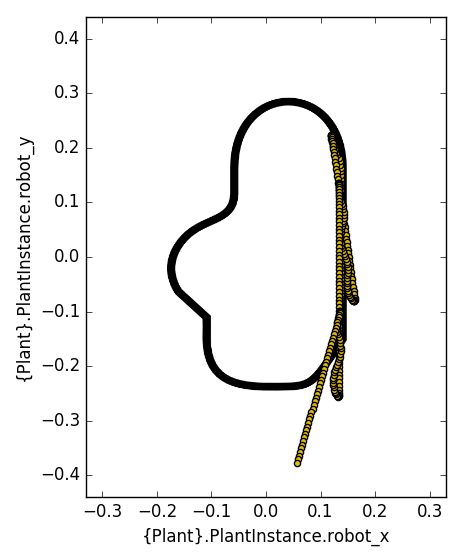
\includegraphics[width=0.5\textwidth]{img/actuator_attack_control.png}
	\caption{Line follower robot path when
	attacked}\label{fig:actuatorcontrolresult}
\end{figure}

In \figref{fig:actuatorcontrolresult} we can see the result of the attack: This
attack can be easily interpreted looking at the figures, the robot go forward
for a period of time and then it go backwards for \code{attack duration}
seconds.


\subsection{Switch Sensors Attack}

This attack is performed by adding a \code{sensor\_attack} function to the
\code{controller} FMU\@.

The attacker can tune the following parameters:
\begin{itemize}
	\item \code{Real attack\_time}: The time at which the attack strats.
	\item \code{Real attack\_duration}: The duration of the attack.
	\item \code{Bool cyclic}: If \code{true} the attack is performed
		periodically.
\end{itemize}

The attack switches the right and left sensors' output, as we can see from
\lstref{lst:switchsensorsatk}.

\lstinputlisting[language=C, label={lst:switchsensorsatk},
caption={Switch sensors attack function}]{switch-sensors-attack-control.c}

We can see from \figref{fig:switchsensorsatkresult} that, when the attack
starts, the robot rotates to the right and gets away from the path. After that,
the robot continues to rotate since it cannot see any line to the right nor to
the left. When the attack ends, the robot manages to get back to the correct
path when it hits against the line again.

\begin{figure}[htb]
	\centering
	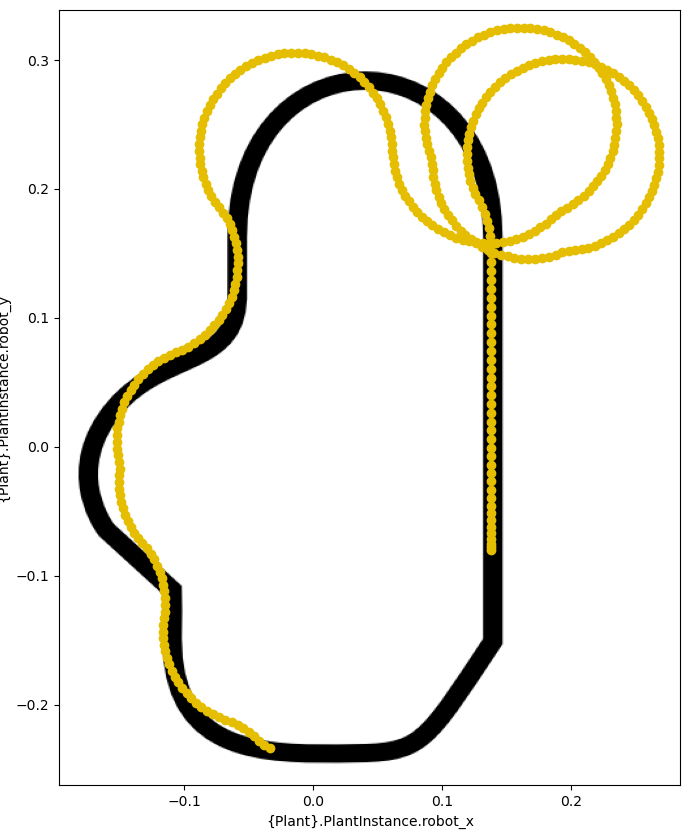
\includegraphics[width=0.5\textwidth]{switch-sensors-attack}
	\caption{Line follower robot path when
	attacked}\label{fig:switchsensorsatkresult}
\end{figure}

\subsection{Complementary Attack}

This attack is carried out adding an extra function to the \code{controller}
FMUs. The attack consists into changing the values coming from sensors with
their complement (\(255 - value\)). This implies that instead of white the
controller sees black and vice-versa (with the exclusion of some readings near
to the colour threshold).

\lstinputlisting[language=C, label={lst:complementary_attack},
caption={Attack algorithm.}]{complementary_attack_ctrl.c}

The attack function for sensors must be placed at the beginning of the regular
controller \code{tick} function.

\begin{figure}[htb]
	\centering
	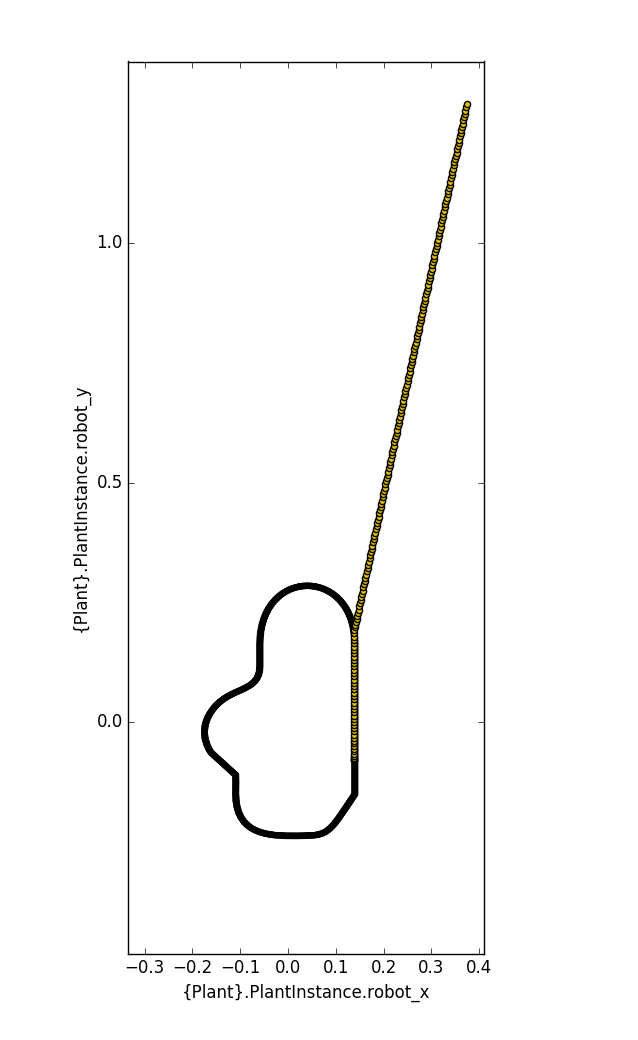
\includegraphics[width=0.5\textwidth]{complementary-attack}
	\caption{Line follower robot path when
	attacked}\label{fig:complatkresult}
\end{figure}

We can see from \figref{fig:complatkresult} that instead of turning left the
robot turns right. It is correct because sensor values are complemented, so the
consequent speed of the wheel is inverted between the two wheels.


\newpage
\section{FMU Attacks}

These attacks are, as said before, carried out using additional malicious FMUs
positioned among the legitimate FMUs. As we can see from the diagram in
\figref{fig:fmuatksdiagram}.

\begin{figure}[htb]
	\centering
	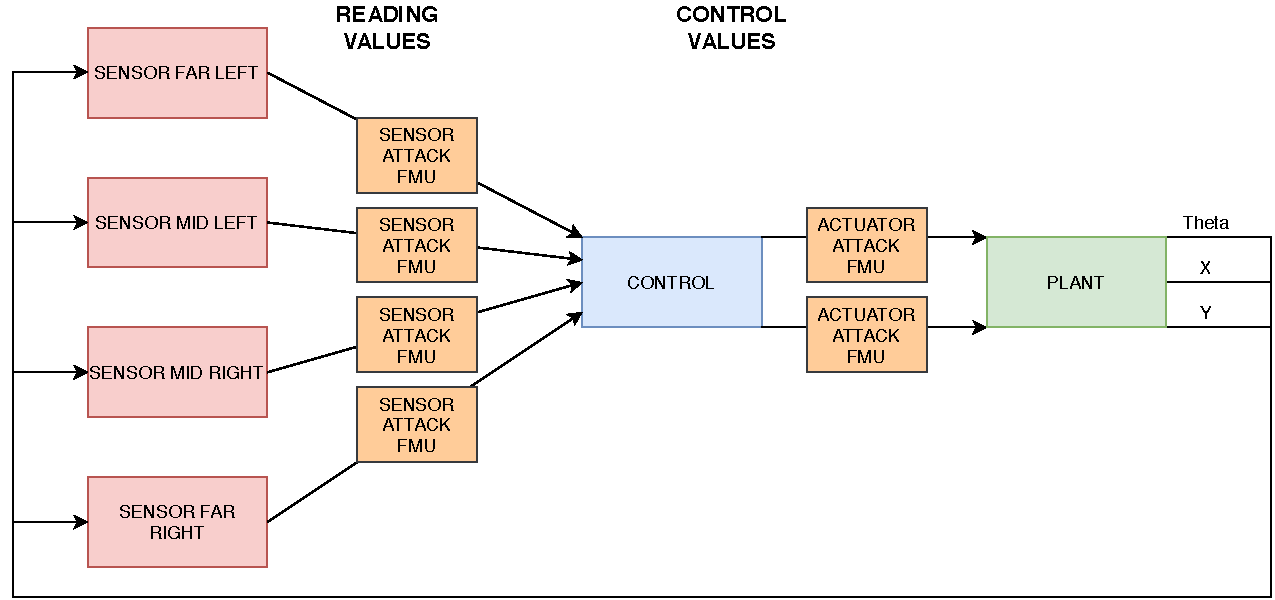
\includegraphics[width=0.77\textwidth]{fmu-attacks-diagram}
	\caption{FMU attacks diagram}\label{fig:fmuatksdiagram}
\end{figure}

In these section we will describe the attacks and discuss the outcomes.

\subsection{Actuator scale attack}
This attack is carried out adding two extra FMUs between the \code{controller}
and the \code{plant} FMUs, one for each output of the \code{controller}.

This attack can be performed in two different ways:
\begin{enumerate}
	\item Interval Mode: In this mode the attack is performed once, for an
		interval of time defined by the attacker, starting from an
		instant chosen from the attacker.
	\item Cyclic Mode: The attack is performed periodically.
\end{enumerate}

The attacker can choose some parameters:
\begin{itemize}
	\item \code{Real attack\_time}: The time at which the attack starts.
	\item \code{Real attack\_duration}: The duration of the attack.
	\item \code{Real attack\_value}: The speed change coefficient.
	\item \code{Bool cyclic}: If \code{true} the attack is performed
		periodically.
\end{itemize}

The objective of the attack is to set the values for the actuators, contained in
the \code{plant} component, so that the robot will go at a different speed from
the right one: from the first half of \code{attack\_duration} the speed is
multiplied by \code{attack\_value}; into the second half of
\code{attack\_duration} the speed is divided by \code{attack\_value}.

\lstinputlisting[language=C, label={lst:scale_attack},
caption={Attack fmu algorithm.}]{actuator_scale_attack_fmu.c}

\begin{figure}[htb]
	\centering
	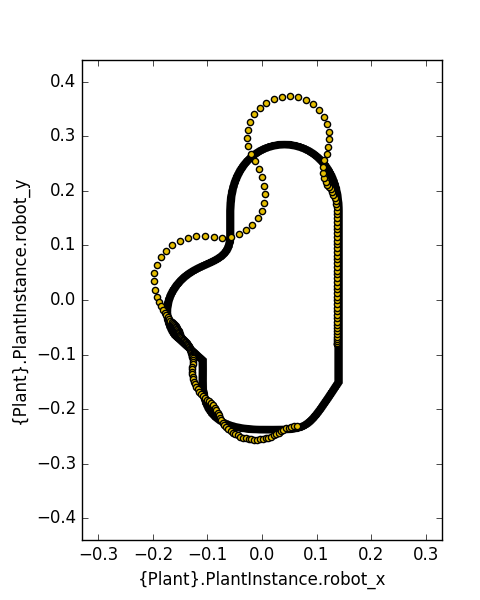
\includegraphics[width=0.5\textwidth]{actuator-scale-attack}
	\caption{Line follower robot path when
	attacked}\label{fig:actuatorscaleresult}
\end{figure}

In \figref{fig:actuatorscaleresult} we can see the result of the attack: in the
first part the robot's curves were very distant from the correct path; instead
in the second part the path is followed with more precision.

\subsection{Max Speed Attack}

This attack is carried out adding two extra FMUs between the \code{controller}
and the \code{plant} FMUs, one for each output of the \code{controller}.

This attack can be performed in two different ways:

\begin{enumerate}
	\item Interval Mode: In this mode the attack is performed once, for an
		interval of time defined by the attacker, starting from an
		instant chosen from the attacker.
	\item Cyclic Mode: The attack is performed periodically.
\end{enumerate}

The attacker can choose some parameters:

\begin{itemize}
	\item \code{Real attack\_time}: The time at which the attack starts.
	\item \code{Real attack\_duration}: The duration of the attack.
	\item \code{Real attack\_value}: The speed at which the actuator should
		drive the motors of the LFR during the attack.
	\item \code{Bool cyclic}: If \code{true} the attack is performed
		periodically.
\end{itemize}

The objective of the attack is to set the values for the actuators, contained in
the \code{plant} component, so that the robot will go at the speed chosen from
the attacker.

The FMU algorithm is shown in \lstref{lst:maxspeedattack}.

\lstinputlisting[language=C, label={lst:maxspeedattack},
caption={Attack fmu algorithm.}]{max_speed_attack.c}

\begin{figure}[htb]
	\centering
	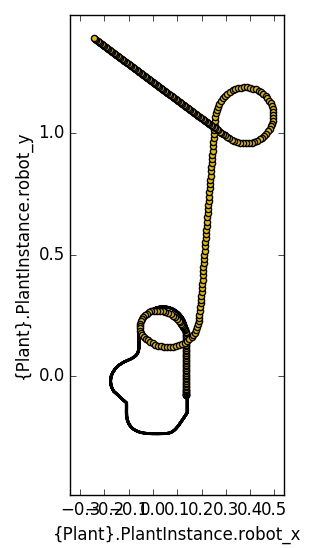
\includegraphics[width=0.5\textwidth]{max_speed_attack.png}
	\caption{Line follower robot path when
	attacked}\label{fig:maxspeedresult}
\end{figure}

In \figref{fig:maxspeedresult} we can see the result of the attack: the FMUs are
activated one at a time, so the robot will turn left since the right FMU is
attacked earlier, then it will go straight, and it will turn right again, since
the right attack FMU stops injecting attack values. In the last part of the
figure we can see the robot going straight, this can be explained looking at the
last legitimate value for the actuators before the attack started.

\subsection{Sensors Output Attack}

\ldots



